%% ****** Start of file apstemplate.tex ****** %
%%
%%
%%   This file is part of the APS files in the REVTeX 4 distribution.
%%   Version 4.1r of REVTeX, August 2010
%%
%%
%%   Copyright (c) 2001, 2009, 2010 The American Physical Society.
%%
%%   See the REVTeX 4 README file for restrictions and more information.
%%
%
% This is a template for producing manuscripts for use with REVTEX 4.0
% Copy this file to another name and then work on that file.
% That way, you always have this original template file to use.
%
% Group addresses by affiliation; use superscriptaddress for long
% author lists, or if there are many overlapping affiliations.
% For Phys. Rev. appearance, change preprint to twocolumn.
% Choose pra, prb, prc, prd, pre, prl, prstab, prstper, or rmp for journal
%  Add 'draft' option to mark overfull boxes with black boxes
%  Add 'showpacs' option to make PACS codes appear
%  Add 'showkeys' option to make keywords appear
\documentclass[aps,prl,reprint,groupedaddress]{revtex4-1}
%\documentclass[aps,prl,preprint,superscriptaddress]{revtex4-1}
%\documentclass[aps,prl,reprint,groupedaddress]{revtex4-1}

% You should use BibTeX and apsrev.bst for references
% Choosing a journal automatically selects the correct APS
% BibTeX style file (bst file), so only uncomment the line
% below if necessary.
%\bibliographystyle{apsrev4-1}
\usepackage{graphicx}
\usepackage{braket}
\usepackage{amsmath}
\usepackage[monochrome]{color}
\begin{document}
% Use the \preprint command to place your local institutional report
% number in the upper righthand corner of the title page in preprint mode.
% Multiple \preprint commands are allowed.
% Use the 'preprintnumbers' class option to override journal defaults
% to display numbers if necessary
%\preprint{}

%Title of paper
\title{Two-Level System Interactions with Superconducting Quantum Circuits}

% repeat the \author .. \affiliation  etc. as needed
% \email, \thanks, \homepage, \altaffiliation all apply to the current
% author. Explanatory text should go in the []'s, actual e-mail
% address or url should go in the {}'s for \email and \homepage.
% Please use the appropriate macro foreach each type of information

% \affiliation command applies to all authors since the last
% \affiliation command. The \affiliation command should follow the
% other information
% \affiliation can be followed by \email, \homepage, \thanks as well.
\author{John Rinehart\\
\normalsize QIC 880 Nanoelectronics Quantum Information Processing}
\email{jrinehar@uwaterloo.ca}
%\homepage[]{Your web page}
%\thanks{}
%\altaffiliation{}
\affiliation{University of Waterloo}

%Collaboration name if desired (requires use of superscriptaddress
%option in \documentclass). \noaffiliation is required (may also be
%used with the \author command).
%\collaboration can be followed by \email, \homepage, \thanks as well.
%\collaboration{}
%\noaffiliation

\date{\today}

\begin{abstract}
Two-level systems are a major source of decoherence for superconducting circuits. Experimental evidence has radically altered the contemporary theory of the origins of two-level systems. It is the goal of this paper to outline the measurements and corresponding theory that dictate the most modern understanding of two-level systems. An introduction to the historical understanding of quantum two-level systems will be given, followed by a tour through the most conclusive and foundational experimental evidence. To conclude, a ``forensic'' description of the behavior and identifying characteristics of two-level systems will be supplied to the reader.
\end{abstract}

% insert suggested PACS numbers in braces on next line
\pacs{}
% insert suggested keywords - APS authors don't need to do this
%\keywords{}

%\maketitle must follow title, authors, abstract, \pacs, and \keywords
\maketitle

% body of paper here - Use proper section commands
% References should be done using the \cite, \ref, and \label commands
\section{Introduction}
% Put \label in argument of \section for cross-referencing
Two-level systems have been observed experimentally as early as the late 1970s when cryogenic measurements of the electromagnetic properties of glasses were seen to exhibit a sharp deviation from theory (see \cite{von_schickfus_saturation_1977}). Similarly, bulk measurements on the thermodynamic properties of glass in the late 1980s also resulted in attributing deviation from theory on the presence of two-level systems (see \cite{phillips_two-level_1987}). Specifically, macroscopic thermodynamic quantities such as the heat capacity and thermal conductivities of solids were seen to decrease at a different rate than was expected according to theory. In the low-temperature limit materials should exhibit a near-zero heat capacity that decreases linearly with decreasing temperature. However, measurements performed on bulk properties of solids indicated the low-temperature of the solids' heat capacity decreased at a much slower rate than was predicted using the tools of classical mechanics. The explanation given at the time was that there exist irregularities in the structure of the material leading to a non-singular state of the bulk system. The non-singular states of the system arise from the low-temperature, quantum-mechanical behavior of the system since low temperature (read: low energy) systems imply the quantum mechanical behavior of the system. These irregularities, occurring at the microscopic level, allow for the state of the material to tunnel between different potential configurations. In the limit of reasonable uniformity over the bulk material - so the number of defects is not greater than the amount of regular structures - the system can be modeled as many two-level systems tunneling between configurations. The energy responsible for exciting the two-level systems into the higher energy configurations can be explained by thermal interactions between the two-level system and the environment. Equivalently, these excitations can be explained by radiative interactions between the two-level system and the environment. 

Consider a potential configuration as indicated in Fig. \ref{CoupPot} (taken from \cite{phillips_two-level_1987}). Considering the two wells to be sufficiently isolated from one another and considering a particle in the first two levels of the left potential well, $V_1$, and another particle in the first two levels of the right potential well, $V_2$. The joint Hamiltonian describing both particles (which exists in the Hilbert space $\mathcal{H}_1 \otimes \mathcal{H}_2$) can be expressed as $\begin{pmatrix} \frac{E_1}{2} & 0 \\ 0 & \frac{-E_1}{2} \end{pmatrix} \otimes \begin{pmatrix}\frac{E_2}{2} & 0 \\ 0 & \frac{-E_2}{2} \end{pmatrix}$. In the regime where the potentials overlap and $E_2 - E_1$ becomes comparable to the energy barrier between the two wells, the two systems become entangled and the Hamiltonian must be re-evaluated. Considering a small amount of overlap, this Hamiltonian can be expressed as \[ \tilde{H} = \begin{pmatrix} E_1 + \bra{\Phi_1}V-V_1\ket{\Phi_1} & \bra{\Phi_1}H\ket{\Phi_2} \\ \bra{\Phi_2}H\ket{\Phi_1} & E_2 + \bra{\Phi_2}V-V_2\ket{\Phi_2} \end{pmatrix} \]

\begin{figure}%
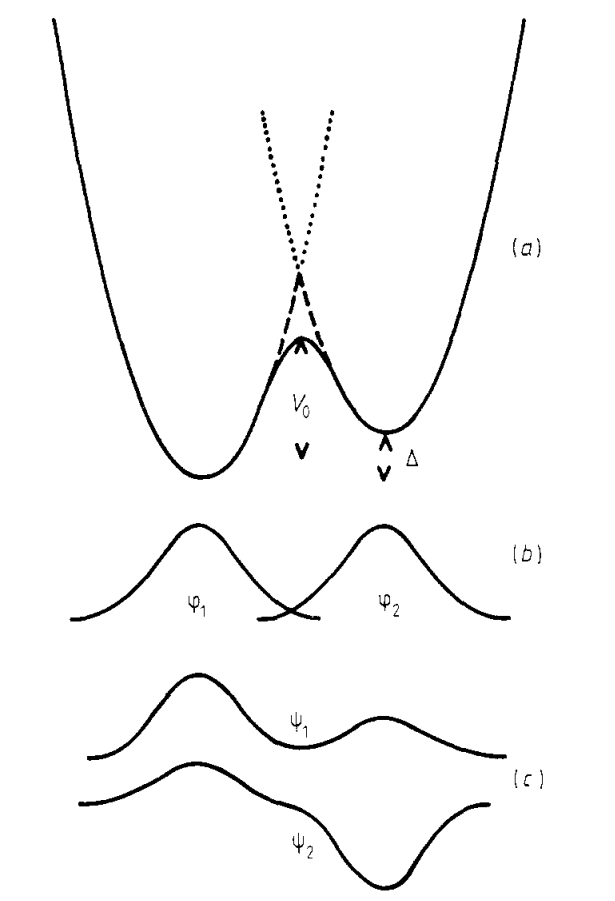
\includegraphics[width=.7\columnwidth,natwidth=615,natheight=901]{../CoupledPotentials.png}%
\caption{Potential Configuration of a Two-Level System. Image from \cite{phillips_two-level_1987}.}%
\label{CoupPot}%
\end{figure}

Such is the standard Hamiltonian of a pair of two-level systems proximal in phase space. The notable characteristic is the coupling of the two systems' energies. Consider the case where a single particle is initially in the ground state of the left well (denoted by the state $\ket{\Psi}=\ket{g_1}$). Allow the right well to be moved through phase space closer to the left well. As the wells begin to overlap it is no longer sufficient to express the state of the particle solely in terms of the one well. In this case, the eigenstates of the new Hamiltonian will be weighted eigenstates of the two wells (the weighting related to the amount of overlap in phase space). The particle's new state is, then, $\ket{\Psi'}=\alpha\ket{g'_1}+\beta\ket{e'_1}$. The energy gap between this new state's two lowest energy levels is larger than it was originally. Furthermore, as depicted in Fig. 1, the, originally, distinct potential energies form an anti-crossing whereby the new potential energy in which the particle resides is not continuous over the energy spectrum but, instead, exhibits a gap in the energy spectrum between two potential energy functions. Considering this new state with respect to the configuration of the potential wells allows for the interpretation that the overlap serves to mediate energy transfer between the left and the right well.

This theory has been used to explain the presence of anomalous two-level systems in the bulk properties of solids (as described previously). These expressions are a direct result of the study of the bulk properties of glass in which many such potential overlaps could occur. In such a situation, only the collective behavior of these defects is visible. However, one could imagine a situation wherein a bulk material is extremely sparsely populated with these two-level system defects. In such a circumstance the behavior of a specific two-level system could be analyzed and characterized. Now, reasoning as to the order of these tunneling energies : At 50 mK the energy of the system is $\sim 4*10^{-6}eV (\sim 1 GHz)$. Realizing that these transitions occur in the microwave regime implies a separate context where two-level systems might be observed in a different light. The immediate application of this new knowledge of two-level systems (its spectral behavior) is to the realm of superconducting circuits.

\section{Experimental Results}

\subsection{Two-Level Systems as Bosonic Dissipators}

In the realm of superconducting circuits, two level systems have been been known to exist for a number of years. Fig. \ref{TLS1}, highlights the presence of several single two-level systems interacting with a prepared qubit state. The signature of the two-level system is the apparent anti-crossing in the energy of the qubit (as described in the Introduction). The method for detecting the set of two-level systems is as follows: 1) Sweep the bias parameters of the qubit until the resonance frequency is found. 2) The resonance frequency being a function of the bias, search for anti-crossings in the excited state of the qubit. It is possible that the two-level system resonance occurs at a resonance of the qubit. In this case, analogous with the potential interaction described in the introduction, the shared energy splitting between the pair of two-level systems results in a transfer of energy from the prepared system (the qubit) to the unprepared system (the two-level system).

\begin{figure}%
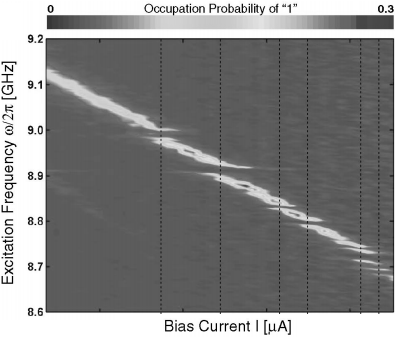
\includegraphics[width=1.1\columnwidth,natwidth=395,natheight=337]{../TLS_Location_SpectroscopyBW.png}%
\caption{Spectroscopy of Qubit Interacting with TLS. Image from \cite{simmonds_decoherence_2004}. }%
\label{TLS1}%
\end{figure}
Although the nature of the two-level system has been discussed in a high-level as an external (unanticipated) system which overlaps with the system of interest in phase space it has not been made explicitly clear what the causes are of the two-level systems. That is, so far no effort has been made to rationalize the natural phenomenon that arises to generate two-level systems at all. The data acquired by Simmonds et. al. in Fig. \ref{TLS1} was accomplished by means of a superconducting quantum interference (SQUID) and a phase qubit. The SQUID and the phase qubit were designed in such a way as to make changes in the current through the Josephson junction of the qubit detectable by the SQUID. Given that the biasing of the qubit results in directly affecting the physical properties of the junction it is reasonable to conclude that the two-level systems arise as a problem with the junction (and not the superconducting traces or the substrate). It is worth noting that Simmonds et. al. made ``experimental checks'' to determine if the coupling of the qubit was to the SQUID responsible for read-out or to the device to which the entire die was mounted.

Beyond detecting anticrossings, Simmonds et. al. measured the coherent oscillations of the qubit in states both on and off resonance with the two-level system. Their claim after measurement was that the two-level system resulted in a reduction of the magnitude of coherent oscillations, not of the energy relaxation time ($T_1$). However, a study of their data set (see Fig. \ref{CohOsc}) seems to offer no reasonable amount of information by which to make a conclusion. 

\begin{figure}%
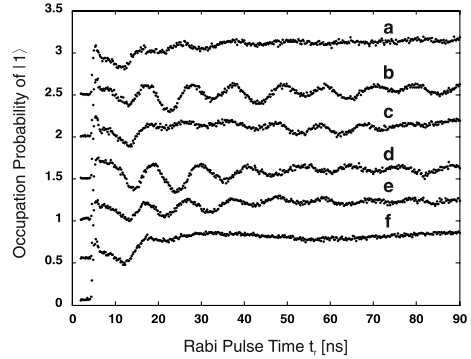
\includegraphics[width=\columnwidth,natwidth=471,natheight=359]{../CohOsc.png}%
\caption{Measurements of the Coherent Oscillation. Image from \cite{simmonds_decoherence_2004}.}%
\label{CohOsc}%
\end{figure}

The explanation given by this group (Simmonds et. al.) was that the two-level systems states were resulting in two separate states of the junction (i.e. two separate critical currents). Thus, the interaction between the junction and the two-level system (TLS) can be expressed in the following form : $\tilde H_{int} = H_{JJ} \otimes H_{TLS} = -\frac{I_A \Phi_0}{2 \pi} \cos(\hat\delta) \otimes\ \ket{\Psi_A}\bra{\Psi_A} - \frac{I_B \Phi_0}{2 \pi} \cos(\hat \delta) \otimes\ \ket{\Psi_B}\bra{\Psi_B} $ . From this point, a 2-level approximation is made of the phase qubit state, the two-level system is represented in its energy eigenbasis and the Hamiltonian takes the simplified form : $H_{int} = \frac{\Delta I_0}{2} \sqrt{\frac{\hbar}{2\omega_{10}}} (\ket{0}\bra{1}\otimes\ket{e}\bra{g} + \ket{1}\bra{0}\otimes\ket{g}\bra{e}$ - where, here, the value $\Delta I_0$ represents the difference between the junction tunneling current when the TLS is in state A minus the tunneling current when the TLS is in state B ($ \Delta I_0 = I_A - I_B$) and $\omega_{10}$ represents the angular transition frequency of the qubit.

Given the form of the interaction Hamiltonian, an expression for the change in the tunneling current relative to the mean can be expressed as : $\gamma = \Delta I_0/ I_0$. These results are listed explicitly in \cite{simmonds_decoherence_2004}. However, they are included here for completeness. Using the magnitude of the measured anti-crossings in the data represented in Fig. \ref{TLS1} allows the value of $\gamma$ to be determined. However, knowing the electrical properties of the junction allows another expression for $\gamma$ to be derived : $\gamma \approx 2\tau R_N e^2/h$. Thus, the alignment of the measured values with theory can be determined. The use of Fig. \ref{TLS1}, in conjunction with the first expression of $\gamma$, Simmonds et. al. obtained a value of $\frac{\Delta I_0}{I_0} \approx 65*10^{-6}$; a prediction of $\gamma$ using the second expression for gamma predicted a value of $8*10^{-6}$. An order of magnitude is a significant margin of error. However, the authors' attempt to explain the discrepancy resulted in attributing the disagreement to the inability of the group to find the largest antisymmetry in the junction and, also, on the limit of the theoretical approach used to obtain the second expression for $\gamma$. However, acknowledging the large disagreement between theory and measured data while positing that the paper likely used a data set that best suited the theory indicates that there likely exists a better (possibly, more complete) description of the physical origin of two-level systems.



\subsection{Two-Level Systems as Fermionic Dissipators}

Measurements very similar to what were performed in \cite{simmonds_decoherence_2004} were performed a year later by Martinis et. al. \cite{martinis_decoherence_2005}. The theoretical approach taken to explain the two-level systems in this paper is markedly different from that taken by Simmonds et. al. in 2004. Whereas the previous theory focused on the two-level system coupling to the current across the junction and allowing energy to be exchanged using the current as the channel, the Martinis theory of 2005 posits that, instead, it is the behavior of an electric dipole toggling between states that is responsible for loss. Initially, this difference may not seem to amount to much expected theoretical difference in the behavior of a two-level system. However, when considering that current-coupling is, fundamentally, a bosonic loss mechanism and that charge-coupling is, likewise fundamentally, a fermionic loss mechanism then a strong asymmetry between the two descriptions of the two-level is strongly implied. The fermionic loss mechanism was documented in works prior to the publication of \cite{martinis_decoherence_2005} (note \cite{von_schickfus_saturation_1977}), however, the expression for the loss was cast into a capacitive form by Martinis et. al. given the geometric nature of the lossy object (a junction). 

The expression for the loss, in this context, can be expressed as \[ \delta(\omega)	 = \frac{\pi\rho(\omega) D^2}{3\epsilon} \frac{\tanh({\frac{\hbar\omega}{2kT}})}{\sqrt{1+\frac{D^2V}{x^2\hbar^2}T_1T_2}} \]

Where D is the strength of the dipole, $\rho$ is the density of states of the two-level systems, $\omega$ is the frequency at which the system is being driven and $\epsilon$ is the dielectric constant of the material, and x is the usual distance between the capacitive plates (in this context, the conductive plates are formed by the superconductors forming the junction).

The loss of the junction can be expressed alternatively by the study of the interaction $H_{int} = \frac{S}{2}(\ket{1}\bra{0}\otimes\ket{g}\bra{e}-\ket{0}\bra{1}\otimes\ket{e}\bra{g})$, where S is the strength of the splitting, $\ket{0}$ and $\ket{1}$ represent the states of the qubit, $\ket{e}$ and $\ket{g}$ represent the state of the qubit (derivation will be omitted for brevity). Then, in a step that is not entirely clear to the author (or to his consultants), the rate of change of the number of splittings over energy and size can be shown to be $\frac{d^2N}{dEdS} = \frac{\sigma A}{S} \sqrt{1-(\frac{S}{S_{max}})^2} $. Now, $\sigma$ is described as a ``materials constant describing the defect density'' effectively implying that the higher the value of $\sigma$ the larger the expected number of defects. Integrating over S, the function can be shown to exhibit logarithmic behavior. Sweeping the parameters $\sigma h$ and $\frac{S}{h}$ Martinis et. al. manage to achieve very good agreement between their results and theory (see Fig. \ref{JunSize}). The solid lines on Fig. \ref{JunSize} indicate the theoretical fit using the chosen values of the parameters $\sigma h$ and $\frac{S}{h}$. It is worth noting that the number of two-level systems purported for the 70 $\mu m^2$ and 13 $\mu m^2$ junctions are due to averages over seven of the larger qubits and four of the smaller qubits. The reason for the asymmetry in the number of tested qubits (four versus seven) is not addressed. 

\begin{figure}%
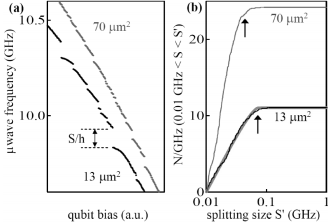
\includegraphics[width=1.4\columnwidth, natwidth=330,natheight=223]{../JunctionSize.png}%
\caption{Scaling of TLS Population with Junction Size. Image from \cite{martinis_decoherence_2005}}%
\label{JunSize}%
\end{figure}

Considering a large number of two-level systems, the next step in the theory reported by Martinis et. al. is to use Fermi's golden rule to obtain an expression for the decay rate in terms of the physical parameters of the junction - again, this is not entirely understood by the author. The end result of such an analysis of a qubit interacting with a multitude of junctions results in a relationship between the energy decay rate $\Gamma_1$ and the physical properties of the junction such that  $\Gamma_1 = \frac{A}{12}(\sigma h) A (S_{max}/h)^2 $. This need not be addressed (given that the result can not be fully justified, here), save that this result has significance when considering that the knowledge of $\sigma h$ and $S_{max}$ from Fig. \ref{JunSize} immediately yield a value that can be expected to be the decay rate of the qubit. Now, the paper continues claiming that using the fitting values ($\sigma h$ and $S_{max}/h$) from Fig. \ref{JunSize} appearing in the previous equation results in a decay rate of $\approx 8 ns$. The author of this paper has substituted their reported fitting values (which are only listed for the 13 $\mu m^2$ case) and did not obtain agreement. It must be the case that the fitting parameters used to obtain agreement were not listed and were also applied to the case of the 70 $\mu m^2$ junction. Note that Martinis et. al. ``attained agreement'' in that the decay rate for the 70 $\mu m^2$ junction's predicted decay rate was close to the decay rate of 186 $\mu m^2$ junctions. The uncertainty can be assigned, at least initially, to the failure of the experiment to conform to the conditions under which the theory was derived. Notably, the simple expression for the decay rate was derived under the assumption that the qubit interacts simultaneously with a bath of two-level systems. However, as depicted in their measured data, the qubit interacts sparsely with two-level systems over the spectrum. This being the case, it can be expected that the actual decay rate $\Gamma_1$ for a qubit of size A would be longer than predicted. Alternatively, the predicted decay rate would be artificially too large and would apply to a qubit that had a larger area. Though this was not noted in \cite{martinis_decoherence_2005}, it does provide qualitative evidence for the discrepancy with theory.

Continuing with the analysis of the 2005 Martinis et. al. publication, it should be apparent that designing the junction with a different material could result in lowering the loss due to the presence of two-level systems. This in mind, Martinis et. al. made measurements of the energy relaxation time (T1) of qubits fabricated with both a $SiO_2$ dielectric and a $SiN_x$ dielectric. The $SiN_x$ samples exhibited an energy relaxation time that was greater than geometrically similar $SiO_2$ samples by a facter of 20. This is indicative of a lower density of two-level systems in the junction (characterized by the parameter $\sigma$ in the theory). These results are shown in Fig. \ref{T1s}.

\begin{figure}%
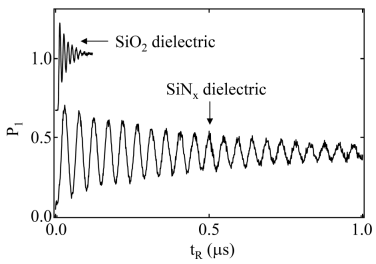
\includegraphics[width=\columnwidth,natwidth=376,natheight=264]{../T1s.png}%
\caption{Measured Energy Relaxation Times for Qubits Utilizing Two Separate Dielectrics. Image from \cite{martinis_decoherence_2005}.}%
\label{T1s}%
\end{figure}

\subsection{Two-Level System Mitigation Techniques}
However, regardless of the bosonic or fermionic nature of the two-level systems one thing is incredibly clear: two-level systems are a material phenomenon. That is, they arise as a byproduct of the deposition of materials needed to fabricate the circuit. This can not be avoided; materials must be deposited. What can be accounted for is the geometry of the circuit elements, the materials used and the deposition technique. It is clear from the literature that a reduction in the size of circuit elements reduces the population of two-level systems by default (there is simply less material in which defects can arise). However, there are physical limits on how small the circuit elements can be fabricated. With regards to this, the next design consideration is the choice of material (substrate and dielectric). As shown earlier, the choice of $SiN_x$ as a substrate material has clear inherent advantages over the use of $SiO_2$. It is worth noting that even though the results comparing $SiN_x$ to $SiO_2$ were published almost a decade ago, $SiN_x$ remains a preferred dielectric to use in the fabrication of Josephson junctions. The last constraint at the disposal of the circuit designer is the deposition technique. Now, typically the deposition of the dielectric is accomplished by means of oxidizing the superconducting metal (forming a dielectric barrier) as in the case of shadow deposition of Josephson junctions. Alternatively, another dielectric may be deposited on top of the superconductor (typically aluminum oxide). It is the case that best results have been found using $SiN_x$, which can be deposited by means of chemical vapor deposition, in place of $SiO_2$ or $AlO_x$.

Now, up until this point, the two-level systems' presence has only been considered in the context of the Josephson junctions. However, the presence of other circuit elements (such as the resonators) are, potentially, another large source of loss. The proper deposition methods and materials for high quality factor resonators have been considered, also. In 2012, Megrant et. al. performed a comprehensive study on various deposition techniques used in the fabrication of superconducting resonators. he material deposited was $Al$ that was subjected to a variety of conditions. Summarized in Fig. \ref{Resons}, it is clear that epitaxied materials perform much better than their sputtered or electron-beam evaporated counterparts. Furthermore, those samples which were annealed (not surprisingly) exhibit much lower internal loss. With these tools in hand the goal of designing a quantum circuit with a higher lifetime becomes that much more accessible.

\begin{figure}%
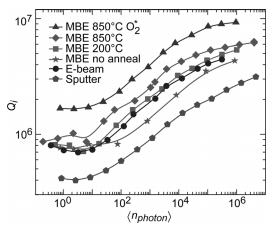
\includegraphics[width=1.3\columnwidth,natwidth=271,natheight=226]{../DepTechsBW.png}%
\caption{Quality Factors of Geometrically-Identical Resonators Varying in Material and Deposition Technique. Image from \cite{megrant_planar_2012}.}%
\label{Resons}%
\end{figure}

\subsection{Overview of Two-Level System Indicators}
Having reviewed the historical theoretical and experimental analysis of two-level systems it is relevant, now, to properly characterize a two-level system. Although the origins of the two-level system have been discussed, the exact character of the two-level system has not been made explicit. Their are several pertinent properties of the two-level system to the experimentalist that, for continuity, have been omitted until now. The purpose of this subsection is simply to enumerate the characteristic signs of a two-level system as indicated in the literature. Some of these properties have already been elaborated on previously, others have not.

\begin{itemize}
	\item Two-level systems when on-resonance with a measurable system will entangle with the measurement system (resulting in energy loss from a prepared system interacting with the two-level system as well as a new set of eigenstates - level-crossing).
	\item Two-level systems affect both the energy decay of a qubit as well as the magnitude of the coherent oscillations (Rabi oscillations) of the qubit. The first of these, the energy decay of the qubit, is widely-documented but, specifically, can be found addressed in \cite{martinis_decoherence_2005}. The second of these, the reduction in coherent oscillation amplitude is addressed in \cite{simmonds_decoherence_2004}. 
	\item Two-level systems are not static in phase space. Characterized as a function of frequency, two-level systems are quasi-stable in time. Spontaneously, (sometimes after days) two-level systems can migrate from a given location in bandwidth to another (possibly disappearing from observation). This is well-documented in the literature and well-known to the designer of quantum circuits. This is a particularly frustrating property of two-level systems.
	\item Two-level systems are relatively stable with regards to temperature variations. As documented in \cite{simmonds_decoherence_2004} and well-known colloquially, each circuit has a sort of ``fingerprint'' that is relatively static as long as the circuit is kept in the superconducting limit. However, a temperature cycle of the circuit (to room temperature and back) has the effect of ``resetting'' the distribution of two-level systems endowing the qubit with a new fingerprint. For this reason, it is not possible to calibrate out the effect of the two-level systems.
	\item Two-level systems seem to appear primarily, though not exclusively, at the interface of two materials. For this reason, materials that are reasonably ``lattice-matched'' need to be selected; also, the deposition method must be relatively robust at maintaining the structural purity of the interface. This design tactic is a direct result of Megrant et. al. in \cite{megrant_planar_2012}.
	\end{itemize}

\section{Conclusion}
There is little left to be said regarding the nature of two-level systems. This review has taken the reader through the solid-state bulk understanding of the nature of two-level systems, the deprecated notion that two-level systems arise as a bosonic noisy channel and the modern (but, possibly incomplete) notion that two-level systems arise as dipole interactions between material defects and the ``ideal'' junction. The study of two-level systems is of vital importance for the circuit designer. It is the understanding of the origins of two-level systems that yields power over their existence. It has been shown that proper selection of materials increases the energy lifetime of the qubit by 20 times, in \cite{martinis_decoherence_2005}. It has been shown that a proper deposition technique increases the quality factor of a resonator by roughly an order of magnitude. These results make apparent that forming a reasonable model of two-level systems allows designers to assuage their prevalence. Thus, after outlining theoretical discussions, practical mitigation techniques were discussed and the intuition behind these results were outlined. Finally, the documented and colloquial properties of two-level systems were outlined for the convenience and immediate reference for the reader.

Note: The reader should not infer that the theory of two-level systems is by any means complete. The physical origin of two-level systems, though contemporarily modeled as a dipole tunneling between available configurations, has not been verified. Experimental evidence, like that in \cite{martinis_decoherence_2005}, has not been shown to be conclusive. What is known is that at least some of the effects of two-level systems can be reduced by adjusting material properties. However, it is yet to be shown that two-level systems can be eradicated completely or that such a task is impossible. 

%\section{\label{}}.
\subsection{}
\subsubsection{}

% If in two-column mode, this environment will change to single-column
% format so that long equations can be displayed. Use
% sparingly.
%\begin{widetext}
% put long equation here
%\end{widetext}

% figures should be put into the text as floats.
% Use the graphics or graphicx packages (distributed with LaTeX2e)
% and the \includegraphics macro defined in those packages.
% See the LaTeX Graphics Companion by Michel Goosens, Sebastian Rahtz,
% and Frank Mittelbach for instance.
%
% Here is an example of the general form of a figure:
% Fill in the caption in the braces of the \caption{} command. Put the label
% that you will use with \ref{} command in the braces of the \label{} command.
% Use the figure* environment if the figure should span across the
% entire page. There is no need to do explicit centering.

% \begin{figure}
% \includegraphics{}%
% \caption{\label{}}
% \end{figure}

% Surround figure environment with turnpage environment for landscape
% figure
% \begin{turnpage}
% \begin{figure}
% \includegraphics{}%
% \caption{\label{}}
% \end{figure}
% \end{turnpage}

% tables should appear as floats within the text
%
% Here is an example of the general form of a table:
% Fill in the caption in the braces of the \caption{} command. Put the label
% that you will use with \ref{} command in the braces of the \label{} command.
% Insert the column specifiers (l, r, c, d, etc.) in the empty braces of the
% \begin{tabular}{} command.
% The ruledtabular enviroment adds doubled rules to table and sets a
% reasonable default table settings.
% Use the table* environment to get a full-width table in two-column
% Add \usepackage{longtable} and the longtable (or longtable*}
% environment for nicely formatted long tables. Or use the the [H]
% placement option to break a long table (with less control than 
% in longtable).
% \begin{table}%[H] add [H] placement to break table across pages
% \caption{\label{}}
% \begin{ruledtabular}
% \begin{tabular}{}
% Lines of table here ending with \\
% \end{tabular}
% \end{ruledtabular}
% \end{table}

% Surround table environment with turnpage environment for landscape
% table
% \begin{turnpage}
% \begin{table}
% \caption{\label{}}
% \begin{ruledtabular}
% \begin{tabular}{}
% \end{tabular}
% \end{ruledtabular}
% \end{table}
% \end{turnpage}

% Specify following sections are appendices. Use \appendix* if there
% only one appendix.
%\appendix
%\section{}

% If you have acknowledgments, this puts in the proper section head.
%\begin{acknowledgments}
% put your acknowledgments here.
%\end{acknowledgments}

% Create the reference section using BibTeX:
\bibliography{FinalPaperReferences}

\end{document}
%
% ****** End of file apstemplate.tex ******

